\documentclass[tikz,border=6pt]{standalone}
\usepackage[T1]{fontenc}
\usepackage{lmodern}
\usepackage{amsmath,amssymb}
\usetikzlibrary{positioning,arrows.meta,fit,calc}
% Design of koblitz-n83-rotkey-20261019 (frozen protocol.json). Not a result.
\begin{document}
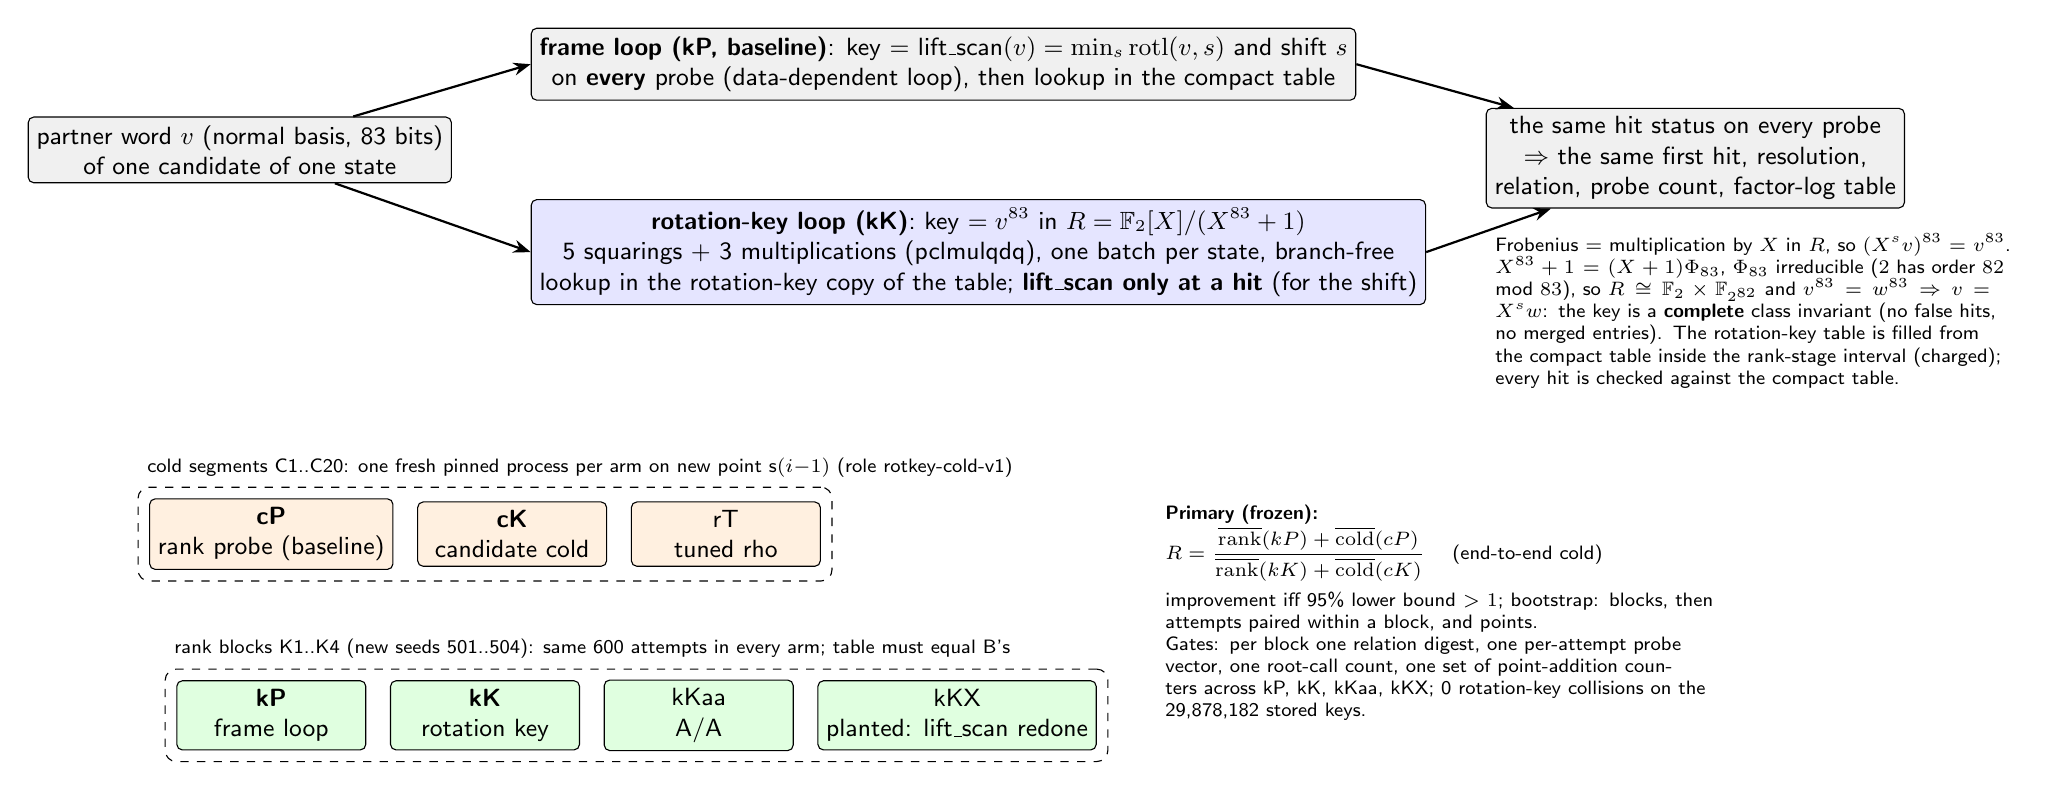
\begin{tikzpicture}[
  font=\sffamily\small,
  box/.style={draw, rounded corners=2pt, align=center, minimum height=8mm, inner sep=3pt},
  base/.style={box, fill=gray!12},
  add/.style={box, fill=blue!10},
  arm/.style={box, fill=orange!12, minimum width=24mm},
  rank/.style={box, fill=green!12, minimum width=24mm},
  arr/.style={-{Stealth[length=2.2mm]}, thick},
  note/.style={align=left, font=\sffamily\scriptsize}
]
\node[base] (in) {partner word $v$ (normal basis, 83 bits)\\of one candidate of one state};
\node[base, above right=2mm and 10mm of in] (fr) {\textbf{frame loop (kP, baseline)}: key $=$ lift\_scan$(v)=\min_s \mathrm{rotl}(v,s)$ and shift $s$\\
on \textbf{every} probe (data-dependent loop), then lookup in the compact table};
\node[add, below right=2mm and 10mm of in] (rk) {\textbf{rotation-key loop (kK)}: key $=v^{83}$ in $R=\mathbb{F}_2[X]/(X^{83}+1)$\\
5 squarings + 3 multiplications (pclmulqdq), one batch per state, branch-free\\
lookup in the rotation-key copy of the table; \textbf{lift\_scan only at a hit} (for the shift)};
\draw[arr] (in) -- (fr.west); \draw[arr] (in) -- (rk.west);
\node[base, anchor=west] (same) at ($(fr.east)!0.5!(rk.east) + (12mm,0)$) {the same hit status on every probe\\$\Rightarrow$ the same first hit, resolution,\\relation, probe count, factor-log table};
\draw[arr] (fr.east) -- (same); \draw[arr] (rk.east) -- (same);
\node[note, anchor=north west, text width=66mm] (ex) at ($(same.south west)+(0mm,-2mm)$) {Frobenius $=$ multiplication by $X$ in $R$, so $(X^s v)^{83}=v^{83}$.
$X^{83}+1=(X+1)\Phi_{83}$, $\Phi_{83}$ irreducible ($2$ has order $82$ mod $83$), so $R\cong\mathbb{F}_2\times\mathbb{F}_{2^{82}}$ and $v^{83}=w^{83}\Rightarrow v=X^s w$:
the key is a \textbf{complete} class invariant (no false hits, no merged entries). The rotation-key table is filled from the compact table inside the rank-stage interval (charged); every hit is checked against the compact table.};
% Cold arms
\node[arm, below=40mm of in, xshift=4mm] (cP) {\textbf{cP}\\rank probe (baseline)};
\node[arm, right=3mm of cP] (cK) {\textbf{cK}\\candidate cold};
\node[arm, right=3mm of cK] (rT) {rT\\tuned rho};
\node[draw, dashed, rounded corners, fit=(cP) (rT), inner sep=4pt, label={[note, anchor=south west]north west:{cold segments C1..C20: one fresh pinned process per arm on new point s$(i{-}1)$ (role rotkey-cold-v1)}}] (cold) {};
% Rank arms
\node[rank, below=14mm of cP] (kP) {\textbf{kP}\\frame loop};
\node[rank, right=3mm of kP] (kK) {\textbf{kK}\\rotation key};
\node[rank, right=3mm of kK] (kKaa) {kKaa\\A/A};
\node[rank, right=3mm of kKaa] (kKX) {kKX\\planted: lift\_scan redone};
\node[draw, dashed, rounded corners, fit=(kP) (kKX), inner sep=4pt, label={[note, anchor=south west]north west:{rank blocks K1..K4 (new seeds 501..504): same 600 attempts in every arm; table must equal B's}}] (rkb) {};
\node[note, anchor=west, text width=70mm] (eq) at ($(rkb.east)+(6mm,13mm)$) {\textbf{Primary (frozen):}\\
$R = \dfrac{\overline{\mathrm{rank}}(kP) + \overline{\mathrm{cold}}(cP)}{\overline{\mathrm{rank}}(kK) + \overline{\mathrm{cold}}(cK)}$ \quad (end-to-end cold)\\[1mm]
improvement iff 95\% lower bound $>1$; bootstrap: blocks, then attempts paired within a block, and points.\\
Gates: per block one relation digest, one per-attempt probe vector, one root-call count, one set of point-addition counters across kP, kK, kKaa, kKX; 0 rotation-key collisions on the 29,878,182 stored keys.};
\end{tikzpicture}
\end{document}
